\section{Präliminarien}
\subsection{Komplexe Zahlen}
Wenn man mit den reelen Zahlen arbeitet, bekommt man Probleme, wenn man die Wurzel aus einer negativen Zahl zieht. Jedoch haben Mathematiker im 17. Jahrhundert eine Lösung dafür entdeckt, indem wir unser Zahlensystem mit den imaginären Zahlen, die die imaginären Einheit i haben, erweitern(Geschichte des Zahlenbegriffs 1970, S.66). Addieren und Subtrahieren zweier imaginären Zahlen funktioniert genau gleich, wie wenn man mit einer Variabel rechnet. Dies heisst, dass man das i wie ein $x$ beim Formeln vereinfachen behandeln kann. Jedoch beim Multiplizieren, Dividieren und beim somit entstehenden Rechnen mit Potenzen muss man aufpassen, denn es gilt für $n \in \mathbb{Z}$:
% Gleichunugen
\begin{align*}
 \text{i}^{4n} &= 1 \\
\text{i}^{4n+1} &= \text{i} \\
\text{i}^{4n+2} &= -1 \\
\text{i}^{4n+3} &= -\text{i}
\end{align*}
%Weiter im Text
Hat man einer der Fälle, ist dies dann zu ersetzen. Hier sieht man gut, dass man die Verknüpfung der imaginären Zahlen reel sein kann, wie es auch andersrum war. Wenn man nun eine imaginäre Zahl $\text{i}b$ mit einer reellen Zahl $a$ zusammenaddiert, bekommt man eine komplexe Zahl  $c=a+\text{i}b$ mit dem Realteil $a$ und dem Imaginärteil $\text{i}b$. $a$ und $b$ sind hier reele Zahlen. Beim Addieren für die Komplexe Zahlen $z=a+\text{i}b$ und $w=e+\text{i}f$
\[z+w\]
\[a+\text{i}b+e+\text{i}f\]
\[a+e+(b+f)\text{i}\]
Nun merkt man, dass diese Zahl mit einem Vektor vergleichbar ist, denn um die Zahl darstellen zu können benutzt man die 2-Dimensionale komplexe Ebene (Mathematik - Die faszinierende Welt der Zahlen 2015, S. 144). Daraus schliesst sich, dass komplexe Zahlen 2-Dimensional sind. Schaut man dies in der komplexe Ebene an, fängt der Punkt an, sich scheinbar unkontrolliert herumspringen, folgt jedoch weiterhin logischen Regeln, beim Quadrieren verschiebt sich der Punkt in die positive Drehrichtung(Gegenuhrzeigersinn). Ebenfalls kann, da die Zahl vergleichbar mit einem Vektor ist, den absoluten Betrag der komplexen Zahl $c$ bestimmt werden, welcher mit dem Pythagoras berechnet wird (Ein Weg zur fraktalen Geometrie 1989, S. 22):
\[|c| = |a+\text{i}b| = \sqrt[2]{a^2+b^2}\]

\subsection{Fraktale Geometrie}
\subsubsection{Allgemein}
Um zum Buddhabrot zu kommen, müssen wir noch einen weiteren Begriff klären, das Fraktal.\\ Würde bei einem 3$n$ grossem Strich der mittlere Drittel fehlen, stattdessen der Rest eines gleichseitigen Dreiecks mit der Seitenlänge $n$ dort stehen, hätte man die erste Iteration einer Kochkurve. Würde man nun in die $n$ grosse Striche die gesamte Kochkurve einfügen, muss man dies ab nun immer wieder machen, sodass es schwer vorstellbar wird. Wenn man jedoch in die Kockurve reinzoomt, findet man die Kochkurve immer wieder: ein rekursives Bild oder eben ein Fraktal(Lexikon der Mathemathik - 3 2001, S. 128).\\Man definiert nun das Fraktal als eine Figur, bei der sehr oft Selbstähnlichkeit auffindbar ist, dass heisst, dass das gesamte Fraktal oder Teile davon mehrfach im Fraktal vorkommen und das Fraktal selbst eine gebrochene und somit keine ganzzahlige Dimension besitzt(Mathematik - Die faszinierende Welt der Zahlen 2015, S. 258).\\
\\
%In der Abbildung \ref{fig:Kochkurve} ist die Entstehung der Kochkurve zu sehen.

\begin{figure}[h]
    \centering
    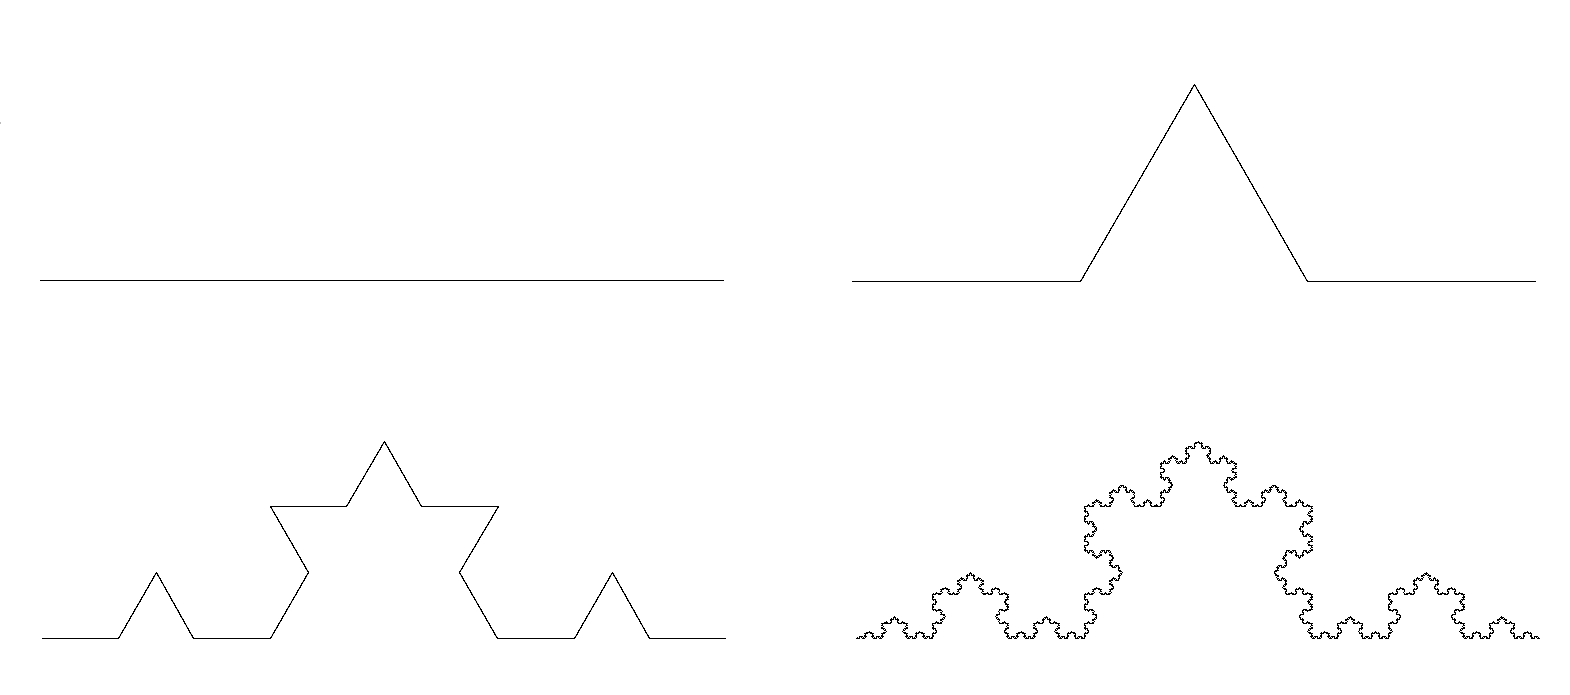
\includegraphics[width=.5\textwidth]{Pictures/Kochkurve.png}
    \caption{Die Enstehung der Kochkurve}
    \label{fig:Kochkurve}
\end{figure}

\subsubsection{Mandelbrotmenge}
Die nach dem Mathematiker Benoît B. Mandelbrot (*20.11.1924; †14.10.2010) bennante Menge ($\mathbb{M}$) beinhaltet jede Zahl $c$ die nicht gegen $\infty$ divergiert für folgende Folge(Ein Weg zur fraktalen Geometrie 1989, S. 54):
\begin{align*}
z_0&=0\\
z_{n+1}&=z^2_n+c
\end{align*}
Man fand heraus, dass wenn $|z_n| > 2$ gilt, wird die Folge gegen $\infty$ divergieren(Ein Weg zur fraktalen Geometrie 1989, S. 74).\\
Das erstellte Bild, mit ein bisschen Farbe jenachdem dazu, ergibt es ein sehr schönes Gebilde, dass den deutschprachigen Leute aufgrund der Form an einem 'Apfelmännchen' errinerte, weshalb es so auch genannt wird(Ein Weg zur fraktalen Geometrie 1989, S. 54).\\
Das $\mathbb{M}$ ist ein Fraktal(Mathematik - Die faszinierende Welt der Zahlen 2015, S. 258). Man findet das erst gesehen Bild der Menge beim reinzoomen immer wieder, somit ist es ebenfalls selbstähnlich. Ebenfalls findet man immer wieder mal verschiedene Julia Mengen mit dem Zugehörigem $c$(Ein Weg zur fraktalen Geometrie 1989, S. 54). Diese sind ebenfalls Fraktale und sehen dazu auch noch für die Norm der Menschheit schön aus. $\mathbb{M}$ besitzt durch die vorgegebene Formel ein chaotisches System(Ein Weg zur fraktalen Geometrie 1989, S. 32).\\
All dies führt sicher dazu, dass es einige YouTube-Viedeos gab, die einen Zoom in die Menge zeigen, welche auch viel Rechenleistung brauchen.

\subsubsection{Buddhabrot}
Schaut man den Namen als Erstes an, wird gemerkt, dass das Wort 'Buddha' vom meditierendem Buddha kommt, den dieser ist in der Abbildung ersichtlich. Ebenfalls das Wort Brot fällt auf, dies ist eine Andeutung, dass diese Abbildung etwas mit dem Mandelbrot zu tun hat, denn es ist eine andere Variante die $\mathbb{M}$ darzustellen\\ 
Das Bild entseht, indessen das Mandelbrot nochmals berechnet wird, jedoch nur die Punkte, die bei der Mandelbrotberechnung gegen das $\infty$ divergieren. Nun wird auch nicht mehr geschaut nach wievielen Schritten es ins $\infty$ abdriftet, sondern bei welchen Punkten es nach jeder Iteration landet.\\
Ebenfalls durch das chaotische System von $\mathbb{M}$ und die fraktalen und selbstähnlichen Eigenschaften, wird ein Zoom in das Buddhabrot intressant.